\section{Discussion}\label{sec:discussion}

In the following, first the experimental results are discussed, and the research questions addressed. Each step of FlowCoder's methodology is analyzed and compared, while including discussions of limitations and strategies for improvement.
Next, we delve into more conceptual aspects of the model, discussing world models, the formation and representation of concepts, causality, the alignment of FlowCoder in a \acrshort{lot}, and finally its integration in a dual processing theory paradigm. 

\subsection{FlowCoder}

\paragraph*{Experiments}


\nameref{sec:exp1} (\autoref{sec:exp1}) suggests that FlowCoder is able to generalize to \acrlong{ood} tasks, given enough sleep. The model solves more tasks in inference than in training, including tasks of groups which had previously been unseen. Offline training, i.e. training on tasks from the generative model, and on remembered task-program pairs is indeed a crucial component of the model, facilitating generalization. This is especially apparent in comparison with experiment 2, in which the sleep phase was substantially reduced and the model performed worse on generalization. However, the sleep phase in experiment 1 was quite excessive and slowed the model down. It is therefore crucial to optimize the sleep phase and to find a balance between the gain of sleep and the cost of computation.

\nameref{sec:exp2} (\autoref{sec:exp2}) shows that the model has learnt the modes of some of the tasks to a degree in which it is able to solve them within one step during inference. As explained in \cite{bengioGFlowNetFoundations2023}, overfitting the model is not an issue, on the contrary, the model is only constrained by the amount of compute going into training. This suggests that when we invest in the model and train it to convergence, we can reap the benefits of the amortized sampler and attain a one-shot inference model.

The experiment shows that on average, the model resamples about 14\% of the programs per task. This highlights an inefficiency of sampling, i.e. until the model learns the reward landscape and samples in proportion to it, it might resample unsuccessful programs. It is especially problematic in tasks that were not solved, meaning that the model is stuck, repeatedly proposing incorrect programs. Better exploration regimes could be employed to encourage a wider exploration of the program space in certain circumstances.
FlowCoder's performance steadily increases with alternating E-M steps, suggesting that it is beneficial to train the generative model separately from the forward policy and having the two models bootstrap each other. The generative model proposes better representations of the program space while the forward policy selects better actions, proportional to the reward function, given the task at hand. This result confirms the findings of \citet{Hu_Malkin_Jain_Everett_Graikos_Bengio_2023}.
In experiment 2, 42 out of 95 tasks were solved during inference. As already mentioned, optimizing the sleep phase may improve the model's performance. 

Additionally, other training regimes should be investigated. In my experiments, FlowCoder attempts to solve the random split of tasks chronologically, meaning the first task is seen with the initial weights of the models, while the last tasks are approached with already somewhat optimized weights. Instead, training on random minibatches of tasks could improve training. Moreover, curriculum learning, i.e. sorting the tasks by difficulty and starting with easier tasks before attempting more difficult ones, could be employed. Another question is for how long to train on a task or how often to switch tasks during training. The hyperparameters of the number of E- and M-steps, number of epochs etc. were decided on empirically, mostly because the experiments were very time consuming, a more rigorous analysis on these details are an interesting topic for future work.

\paragraph*{Minimum Description Length}\label{sec:MDL}
FlowCoder produces diverse solutions. Even in inference it proposes multiple programs solving the tasks, suggesting that it has found a multi-modal distribution. Being able to come up with multiple hypotheses of explaining observations is an important aspect of human cognition. Moreover, humans are able to hold multiple representations of states, exemplified by optical illusions such as the Necker Cube or the Spinning Dancer \footnote{\url{https://en.wikipedia.org/wiki/Necker_cube} and \url{https://en.wikipedia.org/wiki/Spinning_dancer}, respectively}. 
As expected, FlowCoder did not break syntactic symmetries, as shown in \autoref{tab:multiple_solutions}. Many, albeit inefficient, alternate solutions to a task were found. In principle, it is of course useful to avoid multiplying by 1, adding 0, and so on. Breaking syntactic symmetries can be done by favoring programs of minimum description length. DreamCoder does this by including an abstraction phase in which programs are refactored by finding commonalities between similar subroutines \cite{ellisDreamCoderBootstrappingInductive2021}. The authors employ E-graph matching and version spaces — data structures adept at compactly representing alternative iterations of a program and facilitating efficient set operations on these representations, respectively, to manage the combinatorial surge encountered during refactoring. Essentially, the system identifies sub-routines that have proven beneficial across numerous existing and newly discovered programs during the wake phase. It then abstracts these into novel concepts for future tasks, thereby refining and enhancing the \acrshort{dsl}.
\citet{cernaAntiunificationGeneralizationSurvey2023} discuss different approaches for anti-unification, a method for finding generalizable structures between parse-trees. Implementing abstraction, was unfortunately beyond the scope of this thesis.

\paragraph*{Scaling}
The main caveat of my method is that it is slow. Running the experiments took approximately a week and three days, respectively. 
It is somewhat difficult to compare the time efficiency of my method with other approaches for various reasons. 
Both DeepSynth and DreamCoder predict weights for the \acrshort{pcfg} and then parallelize search processes on multiple CPUs. \citet{ellisDreamCoderBootstrappingInductive2021} train DreamCoder for about a day on 20-100 CPUs and it takes around 10 wake-sleep cycles to converge in the list domain, meaning all tasks are solved. Instead, FlowCoder runs on a single GPU (with possible interruptions from other users on the cluster). DreamCoder shows that the refactoring algorithm used in abstraction is crucial in the list processing tasks, which was not implemented in FlowCoder.
The authors of DeepSynth do not include the model query time in their computations and only investigate the performance of different search and sampling strategies. DeepSynth's HeapSearch algorithm solves all tasks, however it creates up to 1.000.000 programs per task, whereas FlowCoder only creates 80.000.
So rather than trying to compare the different algorithms directly, FlowCoder's overall time complexity will be analyzed and whether FlowCoder scales will be discussed, because this is a paramount criterion for a model of cognition. 
\citeauthor{vanrooijTractableCognitionThesis2008}'s \cite{vanrooijTractableCognitionThesis2008} P-Cognition thesis states that cognitive capacities are constrained by tractability - they are limited to functions that can be computed in polynomial time.
The overall strategy I'm employing is to first compile a \acrshort{cfg}, sample rules from it and sequentially form a trajectory, reconstruct the trajectory to \acrshort{ast} format, and lastly evaluate the constructed program. In the following sections, I will analyze these parts in detail, suggest improvements and compare them to other methods.
 
\paragraph*{Rules and Type Inference} \label{par:rules_type}
When using a \acrshort{cfg}, rule look-up can be done in $\mathcal{O}(1)$. Using a \acrshort{cfg} is a nice workaround for my use case but of course human cognition does not come equipped with a \acrshort{cfg}. Instead, when modeling with a typed $\lambda$-calculus, types must be inferred during the \acrshort{ast} construction. Type inference in $\lambda$-calculus can be done in polynomial time \cite{mairsonLinearLambdaCalculus}.
Whether there is a cognitive analogue for a type system remains a point of discussion \cite{ruleChildHacker2020}. \citet{goyalInductiveBiasesDeep2022} show how Transformer's attention can be seen as variable binding, thus implicitly inferring types. This was not investigated in this research because of time constraints but is an interesting topic for future research.

\paragraph*{Program Sampling, Representation, and Embedding}
As outlined in \autoref{sec:sampling_programs}(\nameref{sec:sampling_programs}), FlowCoder constructs programs by sampling rules sequentially. The bulk of the computation is done by the Transformer, specifically the self-attention mechanism, with a time complexity of $\mathcal{O}(n^2)$ per forward pass \cite{keles2022computational}. The auto-regressive trajectory construction therefore has a time complexity of $\mathcal{O}(n^3)$. However, \acrshortpl{ast} can be constructed in various orders. Ideally, additionally to predicting the value of the next node, we could let the GFlowNet predict which node to expand next. However, this would have meant creating an additional model as a node predictor, which increases FlowCoder's complexity. As mentioned in \autoref{sec:gen_model}, graph neural networks could be useful for this purpose. Currently, each rule of the \acrshort{cfg} is embedded, alternatively additional information like parent, child, and argument index could be parameterized explicitly as in DreamCoder. Moreover, type information, depth, or other variables could be encoded in the node representation. 
\citet{allamanis_learning_2018} use Gated Graph Neural Networks to represent both syntactic and semantic information by including data flow and type hierarchy signals. The authors formalize how to turn \acrshortpl{ast} to graphs. \citet{wang2017dynamic} propose a semantic program embedding, learnt from program execution traces. \citet{ibarz_generalist_2022} present a generalist neural algorithmic learner by leveraging \acrshortpl{gnn}. \citet{zhangNovelNeuralSource2019} propose a novel neural \acrshort{ast} representation of source code. \citet{oliveiraAbstractSyntaxGraphs2013} develop abstract syntax graphs (rather than trees) to preserve sharing and recursion within a DSL. After sampling a trajectory, the program is reconstructed to \acrshort{ast} format which can be done in $\mathcal{O}(n)$.
\acrshortpl{gnn} may be a more natural way to represent tree-structured data such as \acrshortpl{ast} and would eliminate the need to format back and forth between linearized and tree representations of \acrshort{ast}. However, \citet{joshi2020transformers} shows that Transformers are actually a special case of \acrshortpl{gnn}, namely they are fully connected graphs. Therefore, I decided to simply use the Transformer architecture as is.

\citet{zhangHippocampalSpatialRepresentations2023} demonstrate evidence for a hyperbolic geometry in the neural representation of space in the Hippocampus. Given that we are working with trees, a hyperbolic space rather than Euclidean, might be beneficial.
\citet{cetinHyperbolicDeepReinforcement2022} show that agents with a hyperbolic representation of latent state space substantially outperform their Euclidean counterparts in deep reinforcement learning benchmark tasks.
\citet{auyespekHyperbolicEmbeddingFinding} confirm that tree-structured data is better represented in hyperbolic space than in Euclidean space.
Similar results are established by \citet{khanHyperbolicRepresentationsSource} and Nickel \& \citet{nickelPoincareEmbeddingsLearning2017}.   
\citet{luHyperbolicFunctionEmbedding2019} propose a hyperbolic function embedding method and show that it is more efficient in terms of computation as well as storage compared to other graph embedding methods.
Nevertheless, after an initial investigation of hyperbolic \acrshort{ast} embeddings, I decided not to pursue this for two reasons. First, because the trees in the experiments are very shallow (up to depth 4), so the nodes are unlikely to overlap in latent space, and second, because I was constrained by time.
However, hyperbolic embedding spaces show promise and should be investigated in the future. 

\paragraph*{Evaluation}
The time complexity of evaluating an \acrshort{ast} is linear ($\mathcal{O}(n)$) with respect to the number of nodes, assuming constant-time operations, such as a simple arithmetic operation or a variable lookup, at each node ($\mathcal{O}(1)$). If the operation at each node involves more complex processes, such as function calls, recursive evaluations, or complex computations, the time complexity can increase. For instance, if a node operation has a complexity of $\mathcal{O}(m)$, then the overall complexity becomes $\mathcal{O}(n \times m)$.
The structure of the \acrshort{ast} can influence the complexity. For instance, in a highly unbalanced tree, certain types of traversals may become less efficient. Again, different \acrshort{ast} representations would therefore be useful to investigate. Since we are working in an executable language, rather than e.g. natural language, the sampling order and \acrshort{ast} representation may affect the performance of the model. Instead of first constructing the tree and then evaluating it, we could predict terminal nodes first in a bottom-up fashion and evaluate the tree (or subtrees) with successive predictions as is done e.g. in the heap-search algorithm \cite{fijalkowScalingNeuralProgram2021}. Other types of information flow could also propagate through the tree, enriching the node embeddings, as previously discussed.

\paragraph*{Levenshtein as Reward}
The Levenshtein edit distance algorithm (\autoref{app:levenshtein}), when implemented using dynamic programming, can be computed with a time complexity of $\mathcal{O}(m \times n)$, where $m$ and $n$ are the lengths of the two input strings. \citet{AndoniKO10} present a near-linear time approximation of the edit distance within a polylogarithmic factor. \\
However, the Levenshtein edit distance is not optimal either. It captures the syntactic difference between the outputs rather than the semantic nuances. Consider the task \texttt{[1,2,3,4] $\rightarrow$ [1,4,9,16]}. The correct program squares each element in the input list. Say the model constructs two programs. Program $f$ cubes the input list, which outputs: \texttt{[1,8,27,64]}. Program $g$ takes the last element of the list and moves it to index 2: \texttt{[1,4,2,3]}. Semantically, $f$ is closer to the correct program since it knows it must map each element in the list to the power of a variable, but it used the wrong variable, whereas $g$ is not similar to the correct program at all. However, the Levenshtein distance would be higher (and thus the reward lower) for the output of $f$.
The Mean Squared Error, Hamming distance, and similar approaches were explored but deemed unfitting and less informative than the Levenshtein distance. Interpreting the output lists as vectors and calculating e.g. a cosine similarity was also considered, however vectors of varying lengths cannot be compared directly and padding the lists would skew the outcome \footnote{See \citet{han2022data} for a summary of the mentioned approaches}.

\subsection{World Model}
In the programming paradigm, the model learns the structure of the world by adhering to the syntactic relations $\cal{S}$ of the \acrshort{dsl} $\cal{D}$ and applying type inference or, as in DeepSynth and FlowCoder, directly from the \acrshort{cfg}. The combination of the \acrshort{cfg} (or alternatively type inference) and the reward $R$ can be seen as an \emph{explicit} world model. 
The Transformer can be seen as a generative model $p_\theta (x, s)$ that learns to map $T(x, s) = z \propto R$, thereby learning an \emph{implicit} world model.
The forward policy $\pi$ can be regarded as an amortized approximation of $R$, a \acrshort{dag} over the state space, and represents a marginal distribution over trajectories leading to programs $\rho$.
In FlowCoder, $R$ is a static heuristic, fairly sufficient in the list editing domain. However, we may ask how it should be represented in a more complex and dynamic environment.
The "Reward-is-Enough" hypothesis by \citet{silverRewardEnough2021} suggests that an agent maximizing a reward while acting on its environment may be sufficient to elicit intelligence and the abilities that are associated with it. \citet{colasAutotelicAgentsIntrinsically2022} argue, that humans develop by intrinsic motivation, i.e. they set their own goals and rewards. The authors define how an agent can set a goal construct which pairs a compact goal representation with a function that measures its achievement. Reward has also been hypothesized to originate in the environment and be a consequence of computing the distance to intrinsic goals \cite{Juechems_Summerfield_2019}. \citet{ruleChildHacker2020} use "hacking" as a metaphor for learning in cognitive development and highlight the importance of intrinsic motivation. A child does not only solve external goals but instead plays, finds sub-goals, and maintains a diverse network of goals. The reward $R$ could in principle reflect a range of values, such as aesthetics, accuracy, usefulness, etc. which is a thrilling direction for future research. 


\paragraph*{Bayesian Models}
\citet{griffithsBayesianModelsCognition} advocate for a hierarchical Bayesian model as a model for cognition.
FlowCoder can be extended to reflect a Bayesian posterior by parameterizing $R_\theta(z|x) = p_\theta(x, z) = p_\theta(z)p_\theta(x|z)$, such that the policy $\pi$ samples in proportion to the posterior distribution. The distribution can be made explicit by using a distributed probabilistic \acrshort{cfg} - a neuralPCFG as introduced in \citet{kimCompoundProbabilisticContextFree2019} and adapted in GFlowNet-EM \cite{Hu_Malkin_Jain_Everett_Graikos_Bengio_2023}.
However, this necessitates computing the marginal likelihood which is challenging. Of course, it can again be approximated by using GFlowNets or other methods. 
DreamCoder marginalizes over a beam of programs for each task.
\acrfull{mcmc} samples from the posterior distribution without computing the marginal likelihood directly. However, they can be slow to converge and have difficulty with mixing modes.
\acrfull{vi} approximates the posterior with a simpler distribution, which is computationally more tractable. It transforms the problem into optimization. See \autoref{app:vi} for a brief comparison between \acrshort{vi} and \acrshortpl{gfn}. \citet{gulwaniProgramSynthesis2017} give a detailed survey and summarization of program synthesis and commonly used methods.

\paragraph*{Energy-Based Models}

Alternatively, as briefly discussed in \autoref{sec:reward} (\nameref{sec:reward}), the world model could also be represented by an \acrlong{ebm}. I will briefly introduce the idea of \acrshortpl{ebm} in the context of our use case and outline the procedure for their application.

The energy function \( E_\theta(x) \) in \acrshortpl{ebm}, as defined by LeCun et al. \cite{lecunTutorialEnergyBasedLearning}, is a real-valued function where \( x \) represents the data and \( \theta \) the model parameters. \acrshortpl{ebm} are designed such that more probable (or desirable) data points are assigned lower energy values, reflecting their likelihood of being from the real distribution. Conversely, less probable data points receive higher energy values, indicating divergence from the expected distribution. \\
The output of the energy function \( E_\theta(x) \) is unnormalized. The probability of data point \( x \) under this model is given by the Boltzmann distribution:
\begin{equation}
    P_\theta(x) = \frac{e^{-E_\theta(x)}}{Z_\theta}
\end{equation}
where \( Z_\theta \) is the partition function. Computing \( Z_\theta \), which is the sum of \( e^{-E_\theta(x)} \) over all possible \( x \), is computationally challenging. Contrastive Divergence (CD), introduced by Hinton \cite{hinton2002training}, provides a practical method to approximate this function through a two-phase process. \\
In our specific case, a task \( x \) is represented by an input-output pair \((x_{\text{in}}, x_{\text{out}})\). In the \emph{positive phase} of CD, we compute the energy of the real task \( E_\theta(x) \), which serves as a baseline measure of task feasibility. The \emph{negative phase} involves sampling a program \( \rho \) using the policy \( \pi_\phi(\rho | x) \), executing \( \rho \) with \( x_{\text{in}} \) to produce a predicted output \( \tilde{x}_{\text{out}} \) (combined as \( \tilde{x} \)), and then computing the energy for this modified task output \( E_\theta(\tilde{x}) \). The discrepancy in energy between the real and predicted outputs is leveraged to refine the EBM:
\begin{equation}    
    \Delta\theta = \eta (\nabla E_\theta(x) - \nabla E_\theta(\tilde{x})) 
\end{equation}
where \( \eta \) is the learning rate. This training process enables the EBM to distinguish between the expected and predicted outputs, thus providing a detailed reward function that enhances the policy's approximation of the posterior distribution.
A significant advantage of using EBMs in this context is their domain-agnostic nature, allowing flexibility in application across various task domains, extending beyond list editing.
The reward function could be optimized further, incorporating evaluations of partial programs, tree-shape, length (e.g. to optimize for MDL), or other features.

The benefit of \acrlong{ebm} over than Bayesian models is that \acrshortpl{ebm} are implicit, meaning we can make less assumptions about the model which makes this method more flexible.

\paragraph*{Biological Plausibility}
In one way or another, probabilistic world models are useful and necessary. \citet{Pouget_Beck_Ma_Latham_2013} present strong evidence that the human brain can represent probabilistic distributions and show how these may be represented in neural circuits. Moreover, they suggest that humans perform probabilistic inference. \\
The predictive processing paradigm and many other associated theories of cognition posit that instead of viewing the brain as a passive data collector, the brain is a query mechanism, primarily engaged in top-down prediction \cite{bottemannePredictiveMindIntroduction2022,caucheteuxEvidencePredictiveCoding2023,mazzagliaFreeEnergyPrinciple2022}. The primary function becomes producing predictions about imminent sensory inputs. What ascends is the prediction error, the mismatch between predictions and actual sensory input.

We also know that movement is organized hierarchically, initiated by the Cortex, after which the Cerebellum compares the intended movement with the actual movement and sends an error message to the Cortex to improve the accuracy of the subsequent movement \cite{kolb2001introduction}. This hints at the Cerebellum's function of representing some kind of prior and being able to compare what is with what ought to be. 
Recent research suggests that the Cerebellum, containing around 50 \% of the brains neurons, may be responsible for more than just motor-action and could represent a world model \cite{silverCognitiveNeuroscienceFunctional2018,Strick_Dum_Fiez_2009, Tee_Taylor_2019}. More research is needed however, to better understand the specialized brain functions and representations.

As I have shown in this research, the line between probabilistic models such as explicit \acrshortpl{pcfg} and using neural networks, such as the Transformer, to represent an implicit world model is blurred. 
\citet{Griffiths_Zhu_Grant_McCoy_2023} propose to refrain from seeing Bayesian models and neural networks as opposing but rather as complimentary approaches to understand cognition, distinguished by \citeauthor{marr1976understanding}'s \cite{marr1976understanding} 3 levels of analysis, where Bayesian models correspond to the computational level and neural networks to algorithmic and implementational levels of analysis. 


\subsection{Concepts}
Both discrete symbolic and continuous sub-symbolic representations may be necessary to understand human cognition.
Symbols limit bandwidth, are robust to noise, and enable re-use for systematic generalization \cite{dehaeneSymbolsMentalPrograms2022, liuDiscreteValuedNeuralCommunication2021}.
Humans do not start out from a blank slate \cite{lakeBuildingMachinesThat2017, pinker2003blank} but rather have some innate abilities for intuitive physics and psychology \cite{ullmanMindGamesGame2017,ullmanTheoryLearningStochastic2012}, and to recognize symmetry and other relations \cite{dehaeneSymbolsMentalPrograms2022}.
Symbols must be grounded and abstracted bottom-up from sensorimotor interaction with an environment \cite{windridgeRepresentationalFluidityEmbodied2018}. 
\citet{garcezNeurosymbolicAI3rd2020} outline how once neural networks are trained, symbols can be extracted. Consider a neural network that learns certain regularities and recognizes that whenever it sees features of type A, features of type B are also present, but features of type C are not. This implicit rule can be made explicit by converting it into symbols: $\forall x A(x) \rightarrow (\exists y B(y) \land \lnot \exists z C(z))$.
\citet{piantadosiComputationalOriginRepresentation2021} demonstrates how to construct a \acrlong{lot} through combinatorial-logic-like language, which is as expressive as $\lambda$-calculus but does not necessitate primitives. This is done via Church Encoding, where primitives are exchanged by higher-order functions. 
\citet{piantadosiComputationalOriginRepresentation2021} asserts that symbols have no inherent meaning, instead, meaning emerges from the dynamic relations between symbols. I.e., only the conceptual role and the dynamics of the symbols define meaning. This perspective aligns with \acrlong{crs}, which posits that meaning and content are derived from the roles symbols play in thought and language. 
Symbols are static, but their distributed representations as compositions of embeddings afford a rich internal structure which may be interpreted as semantics. Therefore, embedding programs may be a crucial aspect to go beyond syntax and learn a semantic grammar, which is an improvement of FlowCoder over DreamCoder.
\citet{doNeuralCircuitsSymbolic2021} explore how the brain can manipulate symbols. They suggest that sequences and neural populations can provide representations that match the requirements for symbols, and that reinforcement learning and Bayesian inference can give the brain the capacity for goal-directed planning. Moreover, they suggest that neural operations can be mapped to $\lambda$-calculus, bridging the gap between connectionism and classical AI and thereby help us understand the circuit mechanism behind manipulating symbols.

The execution of functions within a computational \acrshort{lot} may be necessary for the generation of new knowledge and the expansion of the \acrshort{dsl}. This process involves the construction of complex concepts from basic primitives, akin to the construction of mathematical knowledge from axioms. In other words, every new concept is the result of a computational process, thereby forcing its correctness. Consequently, since every concept is a trajectory, aligning with constructivist principles, when it is integrated into a world model, coherence is assured.

\paragraph*{Causal Models}
Humans are endowed with an intuitive grasp of causality, which functions as the underpinning for both predictive and counterfactual reasoning \cite{lakeBuildingMachinesThat2017}. This enables humans to extrapolate beyond the confines of empirical data, to conjure hypothetical worlds e.g. in imagination, play, and dreaming.
A causal model typically consists of a set of variables and a set of directed edges between these variables, often represented as a \acrshort{dag}. The vertices in this graph denote variables, which, in this context, could be seen as cognitive states. The directed edges signify causal relationships, pointing from cause to effect.
Causal models facilitate interventions, counterfactuals, and causal inference. Intervention is the ability to model the outcome of purposeful changes, represented mathematically as "do" operations  \cite{pearlTheoreticalImpedimentsMachine2018}. For example, if one were to intervene to set $X = x$, the model would enable us to compute the distribution over $Y$ post-intervention.
Counterfactual reasoning allows us to traverse back in time, in a sense, and assess alternative realities — what would have happened to $Y$ if $X$ had been different?
\citet{kicimanCausalReasoningLarge2023} show that \acrshortpl{llm} (particularly GPT-4) are able to \emph{mimic} causality but do not show evidence of real causality. \citet{zecevicCausalParrotsLarge2023} are skeptical of \acrshort{llm}'s causal abilities and show that even when they perform well on causal tasks, they are more likely to learn correlations of causal facts.
Programs are inherently causal and support counterfactual reasoning \cite{chaterProgramsCausalModels2013}. Using the Transformer, being able to represent a rich representation and forcing it to create executable language - programs, may be an efficient strategy that supports causality. For instance, FlowCoder can use imagined data to make inferences about resulting programs.
However, incorporating causality in probabilistic models and neural networks is still an ongoing and somewhat recent field of research and further developments are necessary to compare and contrast how the brain implements it and how we can build models that are truly causal \cite{scholkopfCausalRepresentationLearning2021}.



\subsection{System 1 \& System 2}
\citet{Kahneman11} describes two distinct systems that characterize the dual aspects of human cognition: \\
\emph{System 1} operates automatically and quickly, with little or no effort and no sense of voluntary control. It encompasses intuitive judgments and perceptual associations — it allows for rapid, heuristic-based processing that is often subconscious.
System 1 uses the world model, providing immediate perceptual hypotheses and predictions that guide behavior in a dynamic manner without the need for conscious deliberation.

\emph{System 2} allocates attention to the effortful mental activities that demand it, including complex computations. It is associated with the conscious, rational mind and is deliberate, effortful, and orderly. 
System 2 aligns with the process of the inferential and constructive process of building a trajectory, leading to a program likely to match a given specification.
Adjusting the forward policy is akin to the effortful correction or modulation of System 1's rapid predictions when errors are detected or when more complex reasoning is required.

For example, when learning to play the piano, initial efforts require conscious attention and deliberate practice to master certain phrases (System 2). Over time, as these phrases become internalized, they can be executed more automatically and intuitively (System 1).

Another way of thinking about this by distinguishing \emph{habitual} vs. \emph{controlled} processing where the former is \emph{implicit} and the latter \emph{explicit} \cite{goyalInductiveBiasesDeep2022}.
System 1 is often conceptualized as \emph{procedural}, \emph{parallel}, \emph{continuous}, and \emph{subsymbolic}, whereas System 2 is seen as \emph{declarative}, \emph{sequential}, \emph{discrete}, and \emph{symbolic}. 
There is a growing literature on discussing the necessity and suggesting methods of incorporating System 1 and System 2 \cite{liuDiscreteValuedNeuralCommunication2021,cartuyvelsDiscreteContinuousRepresentations2021,nyeImprovingCoherenceConsistency2021,lecun2022path,matsuoDeepLearningReinforcement2022}.
FlowCoder attempts to take a step in this direction, bridging the gap between the two systems, by learning an implicit world model and learning a forward policy that constructs programs. In a future work, FlowCoder should learn to refactor and abstract programs, and grow its \acrlong{dsl}.







\subsection{Limitations \& Future Work}
FlowCoder is far from perfect. Many tasks were unsolved and only a very shallow tree depth was permitted. 
I will briefly summarize possible optimizations. 
FlowCoder could benefit from better \acrshort{ast} and \acrshort{dsl} representations (see. e.g. \cite{oliveiraAbstractSyntaxGraphs2013, zhangNovelNeuralSource2019}), hyperbolic embedding spaces that are better able to capture tree structures \cite{luHyperbolicFunctionEmbedding2019}, and partial program evaluations, e.g. as is done in the HeapSearch algorithm \cite{fijalkowScalingNeuralProgram2021}.
By including a backward policy, we can relax the order of the sampling strategy and let FlowCoder predict how to expand an \acrshort{ast}.
Moreover, in this research, many important constraints have been relaxed, such as breaking syntactic symmetries, optimizing for \acrlong{mdl}, and growing the \acrshort{dsl}, all of which can be achieved by incorporating abstraction, as is done in \cite{ellisDreamCoderBootstrappingInductive2021}.
FlowCoder's training can be further optimized by improving the balance between wake and sleep phases and improved exploration.
In order to make FlowCoder applicable in other, more complex domains, the reward needs to be improved, e.g. by parameterizing it as an \acrshort{ebm}. Moreover, the model should be tested in domains other than list-editing, incorporating polymorphic types.


\section{Conclusion}
FlowCoder represents a step forward in the field of program synthesis and neurosymbolic \acrshort{ai}, attempting to bridge the gap between the flexibility of neural networks and the precision of symbolic reasoning. 
The use of a Transformer architecture combined with GFlowNet within the FlowCoder framework enables efficient one-shot inference and extrapolation to novel \acrlong{ood} tasks. Moreover, the integration of replay and fantasy techniques enhances the model's learning process, allowing it to retain and refine solutions over time, further improving its performance and generalization abilities. FlowCoder's design, leveraging both explicit and implicit world models, provides a promising approach to program synthesis. However, optimization techniques and extensions to other domains are required. The experiments revealed a trade-off between generalization capabilities and computational costs, particularly during the sleep phase. Future work could focus on optimizing this aspect to achieve a better balance, enhancing the model's efficiency without sacrificing its learning and generalization abilities. The study touches upon the concept of intrinsic motivation and self-generated goals, which could be a fertile ground for further exploration. The discussion highlights the ongoing debate between symbolic and subsymbolic models, touching upon dual-process theories of cognition. Further theoretical research is needed to deepen our understanding of these models' relationship and how they can be effectively combined to create AI that more closely aligns with human cognitive processes.



















% \subsection{\red{Related Work}}
% \begin{itemize}
%     \item apperception engine
%     \item one language to rule them all
%     \item Lenia
%     \item GLOM
%     \item Kissner
%     \item learning concepts with energy functions.
% \end{itemize}

% Lecun integrates system 1 and system 2 in a hierarchical world model
% GLOM



% \begin{itemize}
%     \item Mahowald et al. \cite{mahowald_dissociating_2023}: Deep study on LLMs. they show LLMs alearn hierarchical structure, abstraction. they distinguish between linguistic and functional competence and show that llms sovle the firsrt but not the second. they have a sectins on how llms fail
% \end{itemize}



% An alternative solution is offered by \citet{hintonHowRepresentPartwhole2021}, constructing subsymbolic parse trees, i.e. without the need for explicit rules or syntax.
% \citet{kissnerNeuralSymbolicFrameworkMental2020} presents a neurosymbolic framework. 

% semi-symbolic (arguably transformer) but also capsule networks with which we can make a part-whole hierarchy without symbols. and SPA. 









% \paragraph*{Bayesian Model}

% In DreamCoder the world model is essentially a DSL with weight vector and the inference model is a recognition model:
% - differences:
% marginalizing over beam, enumerative search.


























































% [The Reichenbach Principle, named after philosopher Hans Reichenbach, is a foundational concept in the philosophy of science, particularly in the study of causation. It essentially states that if two events are found to be statistically correlated, then there must exist some causal connection between them. This causal connection can manifest in three forms: either one event causes the other, the second event causes the first, or both events are influenced by a common cause. This principle highlights the difference between mere correlation (statistical association) and causation (a direct or indirect relationship leading to the occurrence of an event).

% The significance of the Reichenbach Principle becomes clear when considering why causal models contain more information than purely statistical ones. Statistical models excel at identifying and quantifying relationships between variables based on observed data. They can tell us, for example, that two variables tend to vary together in a predictable way. However, statistical models don't inherently provide information about the directionality or the underlying mechanism of these relationships – they don't tell us whether one variable causes changes in the other, or if both are influenced by an external factor.

% Causal models, in contrast, are designed to map out these directional relationships. They go beyond mere association to explain how one variable affects another. This is done by incorporating knowledge of the underlying mechanisms and processes that drive the relationships between variables. In a causal model, variables are not just connected; they are linked in a way that specifies how changes in one will lead to changes in another.

% For example, consider the relationship between smoking and lung cancer. A statistical model can show that smoking is correlated with an increased risk of lung cancer, but it doesn't explain why this is the case. A causal model, on the other hand, can illustrate how smoking leads to biological changes in the body that increase the risk of developing lung cancer, thereby providing a more comprehensive understanding of the relationship.

% In summary, the Reichenbach Principle underscores the necessity of seeking causal explanations behind observed correlations. While statistical models are powerful tools for identifying patterns and relationships in data, causal models offer a deeper level of understanding. They provide insights into the mechanisms and processes underlying these patterns, allowing for more accurate predictions, effective interventions, and a richer comprehension of the phenomena being studied.]
% \cite{causal_representation_learning}


% In the programming paradigm we can think of this as finding a program which sees the data, lung cancer, and can infer a program that makes the causal relationship between smoking and outputs lung cancer. 





% Discussing what LLMs are supposed to model, whether approximations are necessary etc. Symbols. \cite{Blank_2023}


















% FlowCoder is a \emph{predictive} model.
% However, more complex cognitive functions may necessitate probabilistic, \emph{explanatory} models. Explanatory models facilitate additional inference on latent variables and in comparison to predictive models infer causal structure rather than only association or correlation \cite{Shmueli_2010}.





























% Tenenbaum argues for the necessity of Hierarchical Bayesian models of cognition.

% Through the lens of Bayesian inference, the brain is conceptualized as a predictive machine. It constantly generates hypotheses or predictions about the world, drawing on past experiences and current sensory data. The brain, rather than simply processing incoming sensory information, actively infers probable causal factors behind this data, effectively reverse-engineering the world. This inferential process is guided by Bayesian principles, where the brain weighs the likelihood of various hypotheses against the evidence presented by sensory inputs. The "prediction error" – the discrepancy between these predictions and actual sensory experiences – becomes a crucial component, informing and refining the brain's model of the world. This is the premise of many Bayesian cognitive models and associated paradigms such as the Free-Energy Principle, (Hierarchical) Predictive Coding, Bayesian Brain Theory, and many other variants \cite{friston_free-energy_2010, friston_world_2021, Ramstead_Kirchhoff_Friston_2020, caucheteux_evidence_2023, Friston_2012, Knill_Pouget_2004}.

% LeCun \cite{Matsuo_LeCun_Sahani_Precup_Silver_Sugiyama_Uchibe_Morimoto_2022} underscores the necessity of causal inference, facilitated by probabilistic graphical models.










% \subsection{\green{Varied Representations}} \label{sec:varied_reps}
% [aristotle - it is a sign of intelligence to be able to entertain a thought without accepting it.]
% Humans interpret the same data in different ways. 
% Optical illusions, like the old woman/young woman or the duck/rabbit images [show link], Necker cube, serve as a metaphor for this phenomenon. They demonstrate how one set of data (the image) can lead to multiple interpretations. In AI, this reflects the system's capacity to process and understand information from multiple perspectives.


% From a Bayesian perspective, this idea relates to the choice between seeking a singular, most probable interpretation (Maximum A Posteriori, or MAP: $\arg max P(z|x)$) and considering a range of possible interpretations (approximating the posterior distribution: $P(z|x)$). The former approach aims for a definitive answer, while the latter embraces uncertainty and variability in the data.

% \begin{itemize}
%     \item having multiple representations of the same thing. e.g. isomorphisms, Fourier/ Laplace transform
%     \item examplified by old woman/ young woman, duck/ rabbit optical iillusion
%     \item In bayesian terms it is the question of whether we infer a point estimate, e.g. maximum a posteriori (MAP) vs trying to approximate the posterior. (Show the Bayesian formula map vs post)
%     \item We can then further ask whether we have one generative model and try to optimize it or if we construct multiple world models in parallel that are constantly competing and renegotiated.
%     \item This is related to identity and essence, when are two concepts the same? when they are isomorphic?
%     \item Necker Cube, dancing girl, etc. (bistable)
%     \item Discuss why it is a useful property of cognition
%     \item Friston explains that a point estimate is not enough \cite{friston_world_2021} 
% \end{itemize}
















































































% Aligning with this theory, \todo{cite myself. maybe shorten this part, it's not really necessary}
% Murphy \cite{murphy2019introduction} distinguishes between deliberate and reactive agents. Reactive agents have four defined "rules" on which they act. \emph{Reflexes} are hard-wired responses to certain stimuli. A knee-jerk reaction. \emph{Taxes} define the movement of an organism towards (or away from) stimuli. An example is the way ants follow a trail by chemotaxis. More complex behaviour is elicited through \emph{fixed-action-patterns}. These consist of a sequence of certain behaviours, usually triggered by some stimulus. A squirrel's nut burying behaviour is an example. Lastly, the \emph{sequencing of innate behaviors} such as a digger wasp's brood-tending is an example of even more complex behaviour. Further, it has been shown how complex behaviour can emerge as an epiphenomenon such as in swarms or ants \cite{franks1989army}. 


















































































































































% %%%%%%%%%%%%%% Models or model free
% Moreover, model-based reinforcement learning has been shown to perform better, while needing much fewer interactions with the environment, than model-free reinforcement learning \cite{kaiser_model-based_2020}, which highlights the benefit of creating an internal model of the world. Other approaches and benefits of model-based architectures have been discussed, see e.g. \cite{ha_world_2018, ramstead_generative_2022}.









% \subsection{\green{Abduction}}
% \todo{self citation}
% How do we come up with the best explanation given partial information and limited resources? This is the problem of abduction, which can be seen as a collective term to both the generation of hypotheses, in which case it is termed \textit{abduction proper}, as well as the justification of hypotheses, also termed \textit{Inference to the Best Explanation (IBE)} \cite{burks1946peirce}.
% The main problem associated with abduction proper is the difficulty of assessing how one generates fitting hypotheses quickly, while ignoring all possible non-sensical hypotheses.
% Inference to the Best Explanation entails: given that we already have a set of candidate hypotheses, how do we pick the best one? Furthermore, how do we define "best"? Kwisthout presents a computational model in which he characterizes "best" as an explanation that maximizes both probability as well as information content while being parsimonious \cite{kwisthout2013most}.

% In the Bayesian framework the marginalization term \( P(x) \) represents the probability of the observed data, and calculating it requires integrating over all possible hypotheses. In practical terms, this means considering how each potential hypothesis might account for every piece of observed data. This is intractable. To manage this challenge, Bayesian approximation methods provide ways to approximate \( P(x) \) without needing to perform exhaustive calculations. One common approach is to use sampling methods, such as Monte Carlo methods, which estimate 
% \( P(x) \) by taking random samples from the probability distributions of the hypotheses. Another approach is variational inference, which approximates the probability distributions with simpler ones that are easier to compute. [sources + for a detailed discussion see section x]. 

% It is common to divide between the generative model and the recognition density.
% In this Bayesian framework, the joint probability \( P(z, x) = P(x \vert z) \cdot P(z) \) is referred to as the generative model that hypothesizes how sensory data are generated by the hidden states of the world \cite{Ramstead_Kirchhoff_Friston_2020}. In other words, it specifies a joint probability distribution over sensory inputs and potential causes of those inputs. These causes can be anything from the presence of objects in the environment to more abstract concepts like social cues.
% The recognition model is an approximation of the posterior \(Q(z \vert x) \approx P(z \vert x) \), the brain's inference about the state of the world given the data.
% [for further discussion see ]























% \subsection{Making Sense of Sensory input}
% Other model of cognition, making sense of sensory input. here the unity condition is highlighted. do we get that by constructivism?

% - In order to make sense of sensory input, we are able to predict, retrodict and impute. But there is more to it. 
% - We are constructing a mental model, a symbolic theory explaining the sensory input. 
% 	- This is necessary but not sufficient. 
% 	- We need *unity*: the constituents of our theory – objects, properties, and atoms – must be integrated into a coherent whole. Specifically, the unity condition requires that the objects are interrelated via chains of binary relations, the properties are connected via exclusion relations, and the atoms are unified by jointly satisfying the theory's constraints.
% 	- Our definition of unity involves four conditions. 
% 		1. *Spatial unity*: all objects must be unified in space via a chain of binary relations.
% 		2. *Conceptual unity*: all concepts must be unified via constraints. 
% 		3. *Static unity*: all propositions that are true at the same time must jointly satisfy the set of constraints. 
% 		4. *Temporal unity*: all the states must be unified into a sequence by causal rules.
% - Introducing the **Apperception Engine** using their own programming language DataLog. It can take any kind of sequence and predict, retrodict and impute.
% - Model making is important and there are differences in the dimensions.
% 	1. Modeling only observed phenomena vs. latent structure
% 		- This model posits significant latent structure, including type signature and latent objects
% 	1. Explicit and symbolic vs. implicit
% 		- This theory is explicit and human readable both in the state representations and transition dynamics.
% 	1. What type of prior knowledge is built into the model 
% 		- inductive bias in the form of language plus the unity conditions, which are domain-independent. Also, it is entirely unsupervised. 



















% \clearpage














% In Bayesian terms, the core objective is to find the posterior distribution of programs given a specific task. This involves determining the probability of a program being the correct solution based on the observed input-output pairs that define the task. However, a significant challenge in this process is the computation of the marginalization term, which is essential for calculating the posterior.

% The posterior distribution represents the likelihood of a program \( \rho \) being the correct solution given a task \( x \), formalized as \( P(\rho | x) \). According to Bayes' theorem, the posterior can be expressed as:

% \begin{equation}
%     P(\rho | x) = \frac{P(x | \rho) P(\rho)}{P(x)}
% \end{equation}

% Here, \( P(x | \rho) \) is the likelihood of observing the task \( x \) given a program \( \rho \), \( P(\rho) \) is the prior probability of the program, and \( P(x) \) is the evidence or marginal likelihood.

% The term \( P(x) \) in the denominator, known as the marginal likelihood or evidence, is particularly challenging to compute. It is defined as the sum of the likelihood over all possible programs:

% \begin{equation}
%     P(x) = \sum_{\rho} P(x | \rho) P(\rho)
% \end{equation}

% This calculation involves summing or integrating over the entire space of possible programs, which is typically vast and often computationally infeasible, especially for complex DSLs and intricate tasks. 

% Moreover, we would like to solve all tasks:

% \begin{equation}\label{eq:margin}
%     \prod_x^X P(x) = \prod_x^X \sum_{\rho} P(x | \rho) P(\rho)
% \end{equation}

% The problem increases in difficulty, when rather than only searching the DSL for programs that solve the tasks, we try to optimize the DSL itself.


% To simplify calculations, we can compute the log-likelihood and move from the product to the sum over tasks:

% \begin{equation}
%     \log \prod_x^X P(x) = \sum_x^X \log \sum_{\rho} P(x | \rho) P(\rho)
% \end{equation}

% The difficulty in computing the marginalization term arises because of (1) high dimensionality, meaning, the space of all possible programs can be extremely large, especially as the complexity of the DSL and primitives increases; and (2) because the likelihood function \( P(x | \rho) \) can be complex and computationally expensive to evaluate for each program \( \rho \). This means that some form of search over the program space is necessary.






























% %%%%%%%%%%%% Bayesian
% Tenenbaum show why hierarchical bayesian models are a good model of cognition. 









% In his recent book "What is ChatGPT doing?", Stephen Wolfram analyses the internal mechanisms of \acrfullpl{llm} such as ChatGPT \cite{wolfram2023chatgpt}.
% LLMs are descendents of the Transformer architecture are trained on massive datasets of text and code. This allows them to learn the statistical relationships between words and phrases, and to generate human-quality text, translate languages, write different kinds of creative content, and answer questions in an informative way.
% Embedding is the process of converting tokens into dense vectors of numbers. These vectors represent the semantic and syntactic information about the tokens. The embedding layer is important for LLMs because it allows them to learn the relationships between tokens in a high-dimensional space.
% Various levels of embeddings are encoded, which gives aggregate words, sentences, paragraphs, etc. positions in this latent space.
% LLMs primarily learn and operate through next token prediction. They use statistical patterns in data to predict language use, context, and meaning, focusing on determining the next word or phrase in a sequence. This predictive training over time leads to a complex internal representation of language, enabling the model to produce responses that are grammatically correct, contextually relevant, and semantically nuanced.
% Wolfram highlights that GPT doesn't have any explicit knowledge of grammar and the parse trees that govern natural language, yet they learn these nested syntax trees implicitly. 
% Nonsense sentences such as Chomsky's famous example "Colorless green ideas sleep furiously" [source], or jabberwocky sentences [source], show that there is more to language than syntax. There seems to be a semantic grammar, which LLM models learn implicitly.
% LLMs, through exposure to vast amounts of text containing conditional and logical structures (e.g., "if X, then Y"), develop an ability to recognize and generate logically coherent sentences. They seem to mimic forms of syllogistic reasoning, as seen in sentences like "All X are Y. This is not Y, so it's not X." (as in "All giraffes are tall. This is not tall, so it's not a giraffe."). 
% It's possible that LLMs have "discovered" syllogistic logic by looking at huge amounts of text. However, when it comes to more sophisticated formal logic, they fail [source], since they learned this implicit logic by correlation and they don't "know" the actual rules of logic.
% The concept space that LLMs navigate can be illustrated through analogies such as "man is to king as woman is to queen." This represents the learnt semantic space, where relationships and associations are encoded in a high-dimensional embedding space. In this space, concepts and words are positioned in such a way that their relative distances and directions encode meaningful relationships, mirroring the complexities of human language and thought.

% + bayesian and NNs may be different levels of explanation
% + the symbols may give causal structure






% \begin{figure}[H]
%     \centering
%     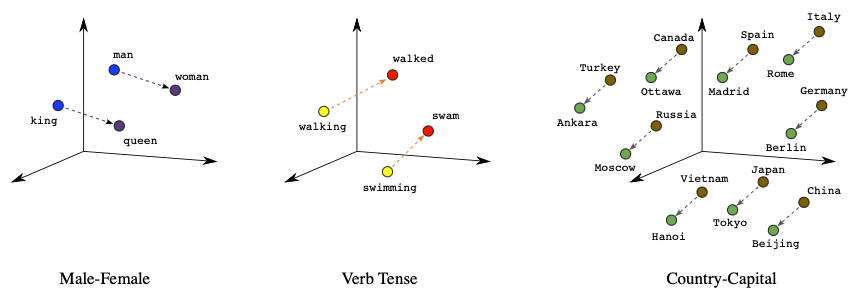
\includegraphics[width=\textwidth]{../img/embeddings_analogies.png}
%     \caption{taken from google}
%     \label{fig:emb_space}
% \end{figure}
% \todo[inline]{Explain the figure, explain vector space, dot product, etc. Discuss the four assumptions under 'shared principles'}










% \rephrase[inline]{from JB: LLMs learn how to complete sequences, they do statistics over patterns}
% Stephen shows that when LLMs create statistics over text, they first discover patterns, then syntax, then style, and only lastly semantics. Humans however start out by discovering semantics and then find patterns, syntax and lastly style. 





































% \subsection{\orange{Comparison to DreamCoder \& DeepSynth}}
% \begin{itemize}
%     \item DC learns a recognition model, giving us a bigram transition matrix. FlowCoder learns a policy. 
%     \item Since we are constructing step-by-step, we are able to start from the middle of a program. 
%     \item MDL
%     \item program embedding + trajectory (step by step construction)
% \end{itemize}

% - how does it work in FC
% - comparison with DC

% - building a DAG (does DC do that?)
% - what does it mean for causality and causal inference?
% - what are benefits of bigram transition matrix vs action policy
% - DC has a weight vector over the DSL which acts as a prior distribution. Q is a recognition model and outputs a bigram distribution so that they can construct programs from it. 
% - In GFN we embed the program as well as the task and output an action. so GFN conditions on the whole trajectory which is encoded in the state while DC only conditions on parent, child, childidx. 
% causality: we would like to apply do-operators, as well as as interventions.
% we want to learn a DAG over ASTs. 
% - is there any difference to outputting a matrix or learning the policy

% - in my method i am embedding programs. this means we can train the model from certain model states, i.e. learning partial program constructions and training from there. we can use foreign programs, akin to someone teaching us how to think e.g. when learning how to derive a proof. 
% then we of course have an actual program space. 

% benefit of my approach is in its enhanced contextual awareness, stemming from the dynamic integration of both task and program state. This could potentially lead to more adaptable and sophisticated program synthesis, enhancing the quality of the policy which takes the need for search. 
% DC is more static, whereas FC adapts the action policy after each step.
% In priciple, we could improve the reward to include the final state and for example optimize for MDL or tree structure or other characteristics of the constructed program.

% DC learns to approximate the posterior during wake. 


% 1. causal inference
% 2. training from the middle, learning a backward policy, subtrajectory balance, etc.
% 3. we are embedding programs, learning additional information and a semantic or concept space
% - we could represent programs and embed differently 
% - hyperbolic space
% - sampling can be done in different strategies
% - then we don't need reconstruction (with complexity O) at all
% - evaluation would also be faster and also inform the NN of partial evaluations
% - additionally we could add data flow etc. 



% In contrast to FlowCoder's and, more generally, GFlowNet's methodology of sequential construction, DreamCoder predicts a transition matrix over the DSL at once. 
% Q is parameterized in such a way that each partial program pp depends on 
% Sequential sampling is beneficial is some regards, though. 

% The input of the forward policy $\pi$ is an encoded state that encapsulates the task as well as a partial trajectory. 

% what does it mean for causality? we can include interventions, counterfactuals, etc. we are building a DAG.
% - with the bigram transition matrix we have a forward and backward policy at once. 

% First, we are training a policy
% However, this is necessary to train the policy and we gain causal inference etc.




























% \begin{itemize}
%     \item benefit over dreamcoder etc. we can ask questions about partial programs. we are embedding programs as well as tasks, we can input a partial program into the model and ask what the next best step is. We can also train from partial tasks etc. making this method more dynamic. [to introduction?]
%     \item As discussed in \autoref{sec:gen_model}, GNNs are  
% \end{itemize}





























































































% Human cognition is inherently hierarchical. We process information at multiple levels – from sensory perception to abstract reasoning. Hierarchical Bayesian models naturally mirror this structure, allowing for the modeling of cognitive processes at various levels of abstraction.
% Human cognition is adept at dealing with uncertainty and ambiguous information. Hierarchical Bayesian models are particularly good at managing uncertainty, as they can integrate prior knowledge with observed data to update beliefs.
% These models facilitate generalization by using higher-level priors that can apply across different contexts. This mirrors how humans apply general knowledge to specific situations.
% Cognitive development involves learning increasingly complex concepts and skills over time. Hierarchical Bayesian models can simulate this learning process, where higher levels of the hierarchy are developed and refined as more data is accumulated.
% Children use prior knowledge when learning about the world, and hierarchical Bayesian models can incorporate such priors effectively, demonstrating how new knowledge builds on existing knowledge.
% Humans have a remarkable ability to understand others' intentions and beliefs (theory of mind). Hierarchical Bayesian models can represent this by considering others' beliefs and intentions at a different level of the hierarchy.
% Human cognition is inherently causal. We often think in terms of causes and effects. Hierarchical Bayesian models can encode causal relationships, making them suitable for modeling how humans infer causality.
% Humans are adept at integrating information from various sources. Hierarchical models facilitate the combination of information at different levels, such as sensory data and high-level conceptual knowledge.
% These models provide a powerful framework for making predictions about future events or unseen data, a core aspect of cognitive processing.
% They offer a coherent computational framework that aligns with many theories of cognition, allowing for precise mathematical modeling and testing of cognitive theories.

% In summary, Tenenbaum highlights hierarchical Bayesian models for cognitive modeling due to their alignment with the hierarchical, flexible, and causal nature of human cognition. These models are capable of handling uncertainty, learning from sparse data, generalizing across contexts, and integrating multiple levels of information, making them particularly suited for exploring the complexities of human thought and learning processes.

% Tenenbaum's work often focuses on integrating the symbolic language of thought with probabilistic models. He suggests that cognition involves not just symbolic processing but also probabilistic reasoning, where beliefs and inferences are updated in a statistically coherent manner.
% In advocating for Bayesian models, Tenenbaum essentially supports a probabilistic language of thought, where symbols and their manipulations are governed by probabilistic rules. This perspective attempts to bridge the gap between symbolic AI and connectionist approaches.





























% \subsection{\green{Compositionality}}
% Humans possess a native capacity for meta-cognitive evaluation, instinctively gauging the reliability of their own knowledge \cite{Lake_Ullman_Tenenbaum_Gershman_2017}. Such self-assessment serves as a compass for learning, steering the acquisition of new information in a manner that refines and optimizes our cognitive architectures.
% Compositionality is central to cognitive productivity and learning. It allows for the creation of infinitely varied representations from a finite set of basic elements, similar to the mind's capacity to think an endless array of thoughts or generate countless sentences. This is particularly useful in forming hierarchical structures that simplify complex relationships, thus making inductive reasoning more efficient.



% State-of-the-art deep-learning models such as large language models are not good at out-of-distribution generalization \cite{Assouel_Rodriguez_Taslakian_Vazquez_Bengio_2022,Xu_Li_Vaezipoor_Sanner_Khalil_2023}.


% deep learning models are of course ultimately compositional. 


% \todo[inline]{should holarchies go here?}







































% The objective is to find parameters that maximize \autoref{eq:margin}, thereby finding


% \begin{equation}
%     \prod_x^X P_\theta(x) = \prod_x^X \sum_{\rho} P_\theta(x | \rho) P_\theta(\rho)
% \end{equation}


% To simplify calculations, we can compute the log-likelihood and move from the product to the log sum over tasks:

% \begin{equation}
%     \log \prod_x^X P_\theta(x) = \sum_x^X \log \sum_{\rho} P_\theta(x | \rho) P_\theta(\rho)
% \end{equation}





% \begin{itemize}
%     \item I don't really marginalize. Instead, I'm using a reward as a heuristic.
% \end{itemize}





% Formally, the overall objective of DreamCoder is to find the optimal DSL \(\mathcal{D}\), which is a set of typed \(\lambda\)-calculus expressions, along with optimal weights \( \theta \) to navigate it, such as to solve a given a set of tasks \(x \in X\).

% I.e. the objective is to find the joint distribution:
% \begin{equation}\label{eq:DC_JD}
%     J(\mathcal{D}, \theta) = P(\mathcal{D}, \theta) \prod_{x \in X} \sum_{\rho} P(x|\rho)P(\rho|\mathcal{D},\theta) 
% \end{equation}

% where:
% \begin{conditions*}
%     P(\mathcal{D}, \theta) & Prior distribution over languages and parameters \\
%     P(x|\rho) & Likelihood of task \(x \in X\) given program \(\rho\)
% \end{conditions*}


% \change{the following doesn't apply anymore?}
% Note the difference to \autoref{eq:margin}. DreamCoder tries not only to find the best programs, but also the optimal DSL, given the tasks. Hence, the dependence on \(P(\mathcal{D}, \theta)\) and \(P(\rho|\mathcal{D},\theta) \).


% Since computing \( J(\mathcal{D}, \theta) \) entails marginalizing over all programs, which is intractable, they instead marginalize over a finite beam of programs per task \( \{\mathcal{B}_x\} \) which is operationalized as a lower bound on the joint density.
% \[
%     \mathcal{L}(\mathcal{D}, \theta, \{\mathcal{B}_x\}) = P(\mathcal{D}, \theta) \prod_{x \in X} \sum_{\rho \in \{\mathcal{B}_x\}} P(x|\rho)P(\rho|\mathcal{D},\theta)
% \]

% The model operates in three distinct phases:

% \begin{description}
%     \item[Wake] In the wake phase, the objective is to find the best program $\rho$ for each task $x \in X$ DreamCoder is presented with. Each task consist of one or a few ($\sim10$) examples.
%     The objective is to maximize \(\mathcal{L}\) w.r.t. to the beam \(\{\mathcal{B}_x\}\)
%     \item[Sleep: Abstraction] A key component of the success of DreamCoder is the refactoring of programs. In this phase, DreamCoder consolidates new abstractions from the programs it has found during the wake phase. Experiences are replayed, and commonalities between programs are found so that they can be abstracted into new concepts to use in the future. 
%     In the abstraction phase \(\mathcal{L}\) w.r.t. \(\mathcal{D}\) is maximized.
%     \item[Sleep: Dreaming] The objective during the dreaming phase is to train the recognition model $Q$ to perform MAP inference by both fantasies, and replays. When fantasizing, programs are drawn from the learned library as a generative model. The model is then trained on the produced tasks. This ensures a large and varied data-set to learn from and encourages out-of-distribution generalization. Replays, simply training on previously seen task-program pairs, ensures that the model improves its predictions on the actual tasks it needs to learn and doesn't forget how to solve tasks it has already solved correctly.
% \end{description}

% In dreaming they maximize \(\mathcal{L}\) w.r.t. \(\theta\).

% \[
%     \mathcal{L}_{\text{MAP}}^{\text{Replay}} = \mathbb{E}_{x\sim X} \left[ \log Q \left( \arg\max_{\rho \in \mathcal{B}_x} P(\rho|x, D, \theta)  \Big\lvert x \right) \right]
% \]

% \[
%     \mathcal{L}_{\text{MAP}}^{\text{Fantasy}} = \mathbb{E}_{x \sim (D, \theta)} \left[ \log Q \left( \arg\max_{\rho} P(\rho|x, D, \theta) \Big\lvert x \right) \right]  
% \]


% The recognition model \(Q\) takes a task as input and outputs a 3-dimensional bigram transition matrix \(Q_{ijk}\), where \(i\) indexes possible children, \(j\) indexes possible parents and \(k\) indexes which argument of the parent is being generated. This parameterization strikes a balance between quality and efficiency.
% The authors chose to optimize MAP rather than the posterior because together with their parameterization of the recognition model, this encourages to break syntactic symmetries.
    


